%**************************************************************************************
% License:
% CC BY-NC-SA 4.0 (http://creativecommons.org/licenses/by-nc-sa/4.0/)
%**************************************************************************************

\documentclass[handout]{beamer}

\mode<presentation> {

\usetheme{Madrid}

% Burnt orange
\definecolor{burntorange}{rgb}{0.8, 0.33, 0.0}
\colorlet{beamer@blendedblue}{burntorange}
% Pale yellow
\definecolor{paleyellow}{rgb}{1.0, 1.0, 0.953}
\setbeamercolor{background canvas}{bg=paleyellow}
% Secondary and tertiary palett
\setbeamercolor*{palette secondary}{use=structure,fg=white,bg=burntorange!80!black}
\setbeamercolor*{palette tertiary}{use=structure,fg=white,bg=burntorange!60!black}

% To remove the footer line in all slides uncomment this line
%\setbeamertemplate{footline}
% To replace the footer line in all slides with a simple slide count uncomment this line
%\setbeamertemplate{footline}[page number]

% To remove the navigation symbols from the bottom of all slides uncomment this line
%\setbeamertemplate{navigation symbols}{}
}

\usepackage{amsmath}
\usepackage{bm}
\usepackage{breqn}
\usepackage{graphicx} % for figures
\usepackage{subcaption} % for subplots 
\usepackage[labelsep=space,tableposition=top]{caption}
\renewcommand{\figurename}{Fig.} 
\usepackage{cleveref}
\usepackage{caption,subcaption}% http://ctan.org/pkg/{caption,subcaption}
\usepackage{booktabs} % Allows the use of \toprule, \midrule and \bottomrule in tables

%----------------------------------------------------------------------------------------
%	TITLE PAGE
%----------------------------------------------------------------------------------------
% The short title appears at the bottom of every slide, the full title is only on the title page
\title[CE394M: Intro to FEM]{CE394M Advanced Analysis in Geotechnical Engineering: FEM} 
\author{Krishna Kumar} % name
\institute[UT Austin] % institution 
{
University of Texas at Austin \\
\medskip
\textit{
  \url{krishnak@utexas.edu}} % Your email address
}
\date{\today} % Date, can be changed to a custom date

\begin{document}

\begin{frame}
\titlepage % title page as the first slide
\end{frame}

\begin{frame}
 % Table of contents slide, comment this block out to remove it
 \frametitle{Overview}
 % Throughout your presentation, if you choose to use \section{} and \subsection{} 
 % commands, these %will automatically be printed on this slide as an overview 
 \tableofcontents
\end{frame}

%----------------------------------------------------------------------------------------
% slides
%----------------------------------------------------------------------------------------

%------------------------------------------------
\section{Introduction to the Finite Element Analysis}
%------------------------------------------------
\begin{frame}
\frametitle{Finite Element Analysis}
 \noindent
\fboxsep=0pt
\noindent
\begin{minipage}[t]{0.42\linewidth}
	\begin{figure}
		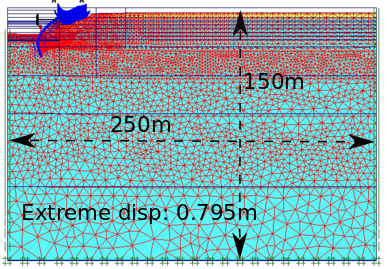
\includegraphics[width=0.95\textwidth]{figs/fea-geotech-mesh.png}
		\caption{FE Mesh}
	\end{figure}
\end{minipage}%
\hfill
\begin{minipage}[t]{0.56\linewidth}
	\begin{figure}
		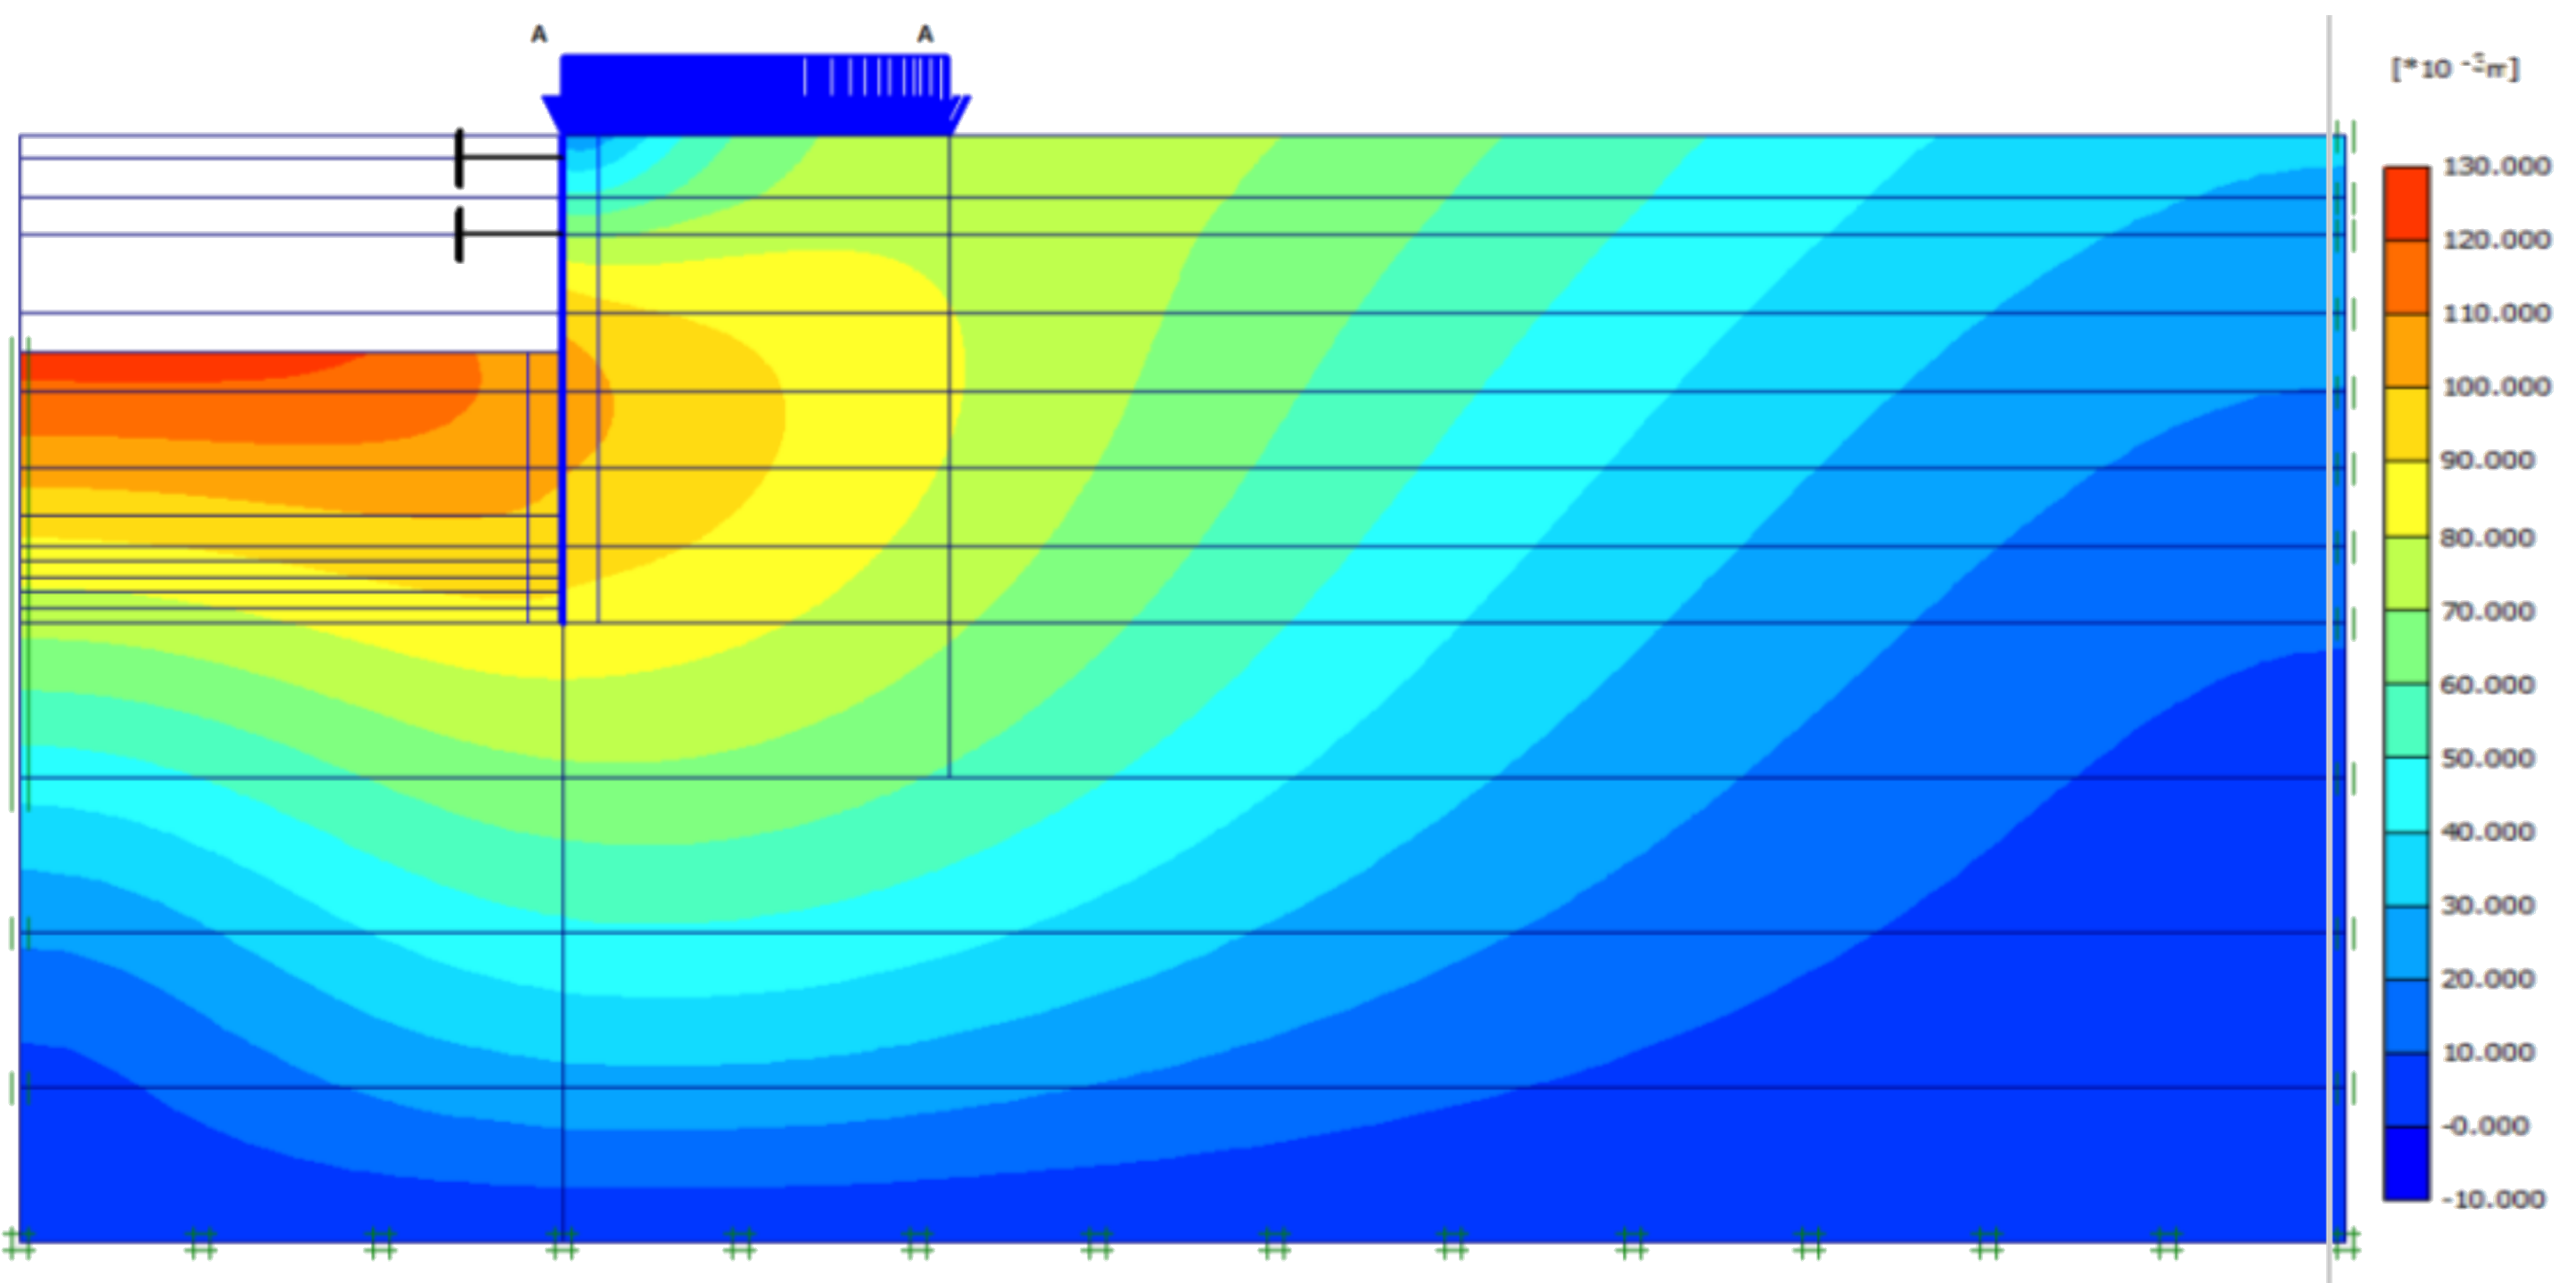
\includegraphics[width=\textwidth]{figs/fea-geotech.png}
		\caption{Displacement profile}
	\end{figure}
\end{minipage}
\centering
Singapore Nicoll highway excavation FE analysis
\end{frame}

%------------------------------------------------
\begin{frame}
\frametitle{Galerkin:Ritz method}
\mode<beamer>{
	\begin{enumerate}
		\item Define the functional $u$ for which you wish to find stationary points.
		\item Choose a combination of linearly independent functions that will be used to approximate the solution. These will be called `basis functions'. The amplitudes of these functions will be the unknowns that you will determine. The basis functions must satisfy the Dirichlet (`fixed') boundary conditions.
		\item Insert the approximate solution into the functional that is now denoted by $u_h$.
		\item Take the directional derivative of $u_h$ with respect to the unknown amplitudes of the
		basis functions.
		\item Determine the amplitudes of the basis functions which yield a stationary point of $u_h$.
	\end{enumerate}
}
\mode<handout>{
	\vspace{5cm}
}
\end{frame}

\note{Numerical methods for partial differential equations are tools for finding approximate
solutions and are normally used with the aid of a computer. A number of numerical
methods are closely linked to a variational form of the differential equation. A group
of such methods are known as Galerkin methods. The Ritz method is an example of a
Galerkin method, and the finite element method is another. If a numerical method is
properly formulated (and the equation is stable), the more effort (read computer time)
that is expended, the closer one gets to the exact solution.}

%------------------------------------------------
\begin{frame}
\frametitle{Finite Element Approximations}
\mode<beamer>{
FE approximation of	$u$, which is a dependent variable in a PDE. 

\begin{figure}[ht]
	\centering
	\begin{subfigure}[b]{0.5\linewidth}
		\centering
		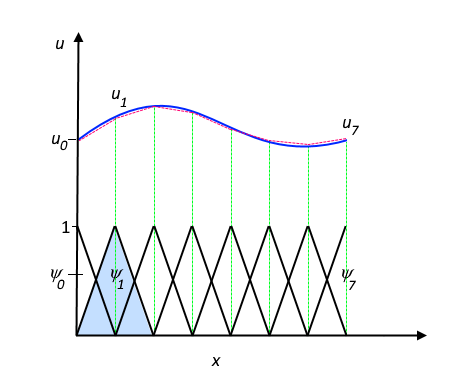
\includegraphics[width=0.8\textwidth]{figs/discretisation2.png}
	\end{subfigure}%
	\begin{subfigure}[b]{0.5\linewidth}
		\centering
		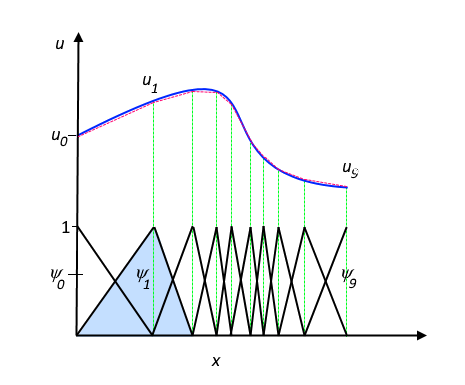
\includegraphics[width=0.8\textwidth]{figs/discretisation1.png}
	\end{subfigure}
	\caption*{FE basis functions}
\end{figure}
The function $u$ can be approximated by a function $u_h$ using linear combinations 
of basis functions according to the following expressions:
\begin{equation*}
u \approx u_h \quad u_h = \sum_{i} u_i \psi_i
\end{equation*}
}
\mode<handout>{
\vspace{5cm}
}
\end{frame}



\note{The reality of partial differential equations is that in most cases it is 
	not possible to find an analytical solution. This is particularly so for 
	equations on complicated geometries (as is common in engineering), nonlinear 
	equations and equations with complicated source terms and boundary conditions.
	
	Instead, an approximation of the equations needs to be constructed, typically 
	based upon different types of discretizations. These discretization methods 
	approximate the PDEs with numerical model equations, which can be solved using 
	numerical methods. The solution to the numerical model equations are, in turn, 
	an approximation of the real solution to the PDEs. The finite element method 
	(FEM) is used to compute such approximations.}

\note{Take, for example, a function $u$ that may be the dependent variable in a PDE 
	(i.e., temperature, electric potential, pressure, etc.) The function $u$ can be 
	approximated by a function uh using linear combinations of basis functions 
	according to the following expressions: 
	
	\begin{equation*}
	u \approx u_h \quad u_h = \sum_{i} u_i \psi_i
	\end{equation*}
	
	Here, $\psi_i$ denotes the basis functions and $u_i$ denotes the coefficients of 
	the functions that approximate u with uh. The figure below illustrates this 
	principle for a 1D problem. $u$ could, for instance, represent the temperature 
	along the length ($x$) of a rod that is nonuniformly heated. Here, the linear basis 
	functions have a value of 1 at their respective nodes and 0 at other nodes. In 
	this case, there are seven elements along the portion of the x-axis, where the 
	function $u$ is defined (i.e., the length of the rod).}

\note{One of the benefits of using the finite element method is that it offers great 
	freedom in the selection of discretization, both in the elements that may be used to 
	discretize space and the basis functions. In the figure above, for example, the elements 
	are uniformly distributed over the x-axis, although this does not have to be the case. 
	Smaller elements in a region where the gradient of u is large could also have been applied.\\
	
	Both of these figures show that the selected linear basis functions include very limited 
	support (nonzero only over a narrow interval) and overlap along the x-axis. Depending on 
	the problem at hand, other functions may be chosen instead of linear functions.\\
	
	\url{https://www.comsol.com/multiphysics/finite-element-method}}


\section{Strong form}

%------------------------------------------------
\begin{frame}
\frametitle{Strong form of the equilibrium equation for a 1-D bar}
\begin{figure}
	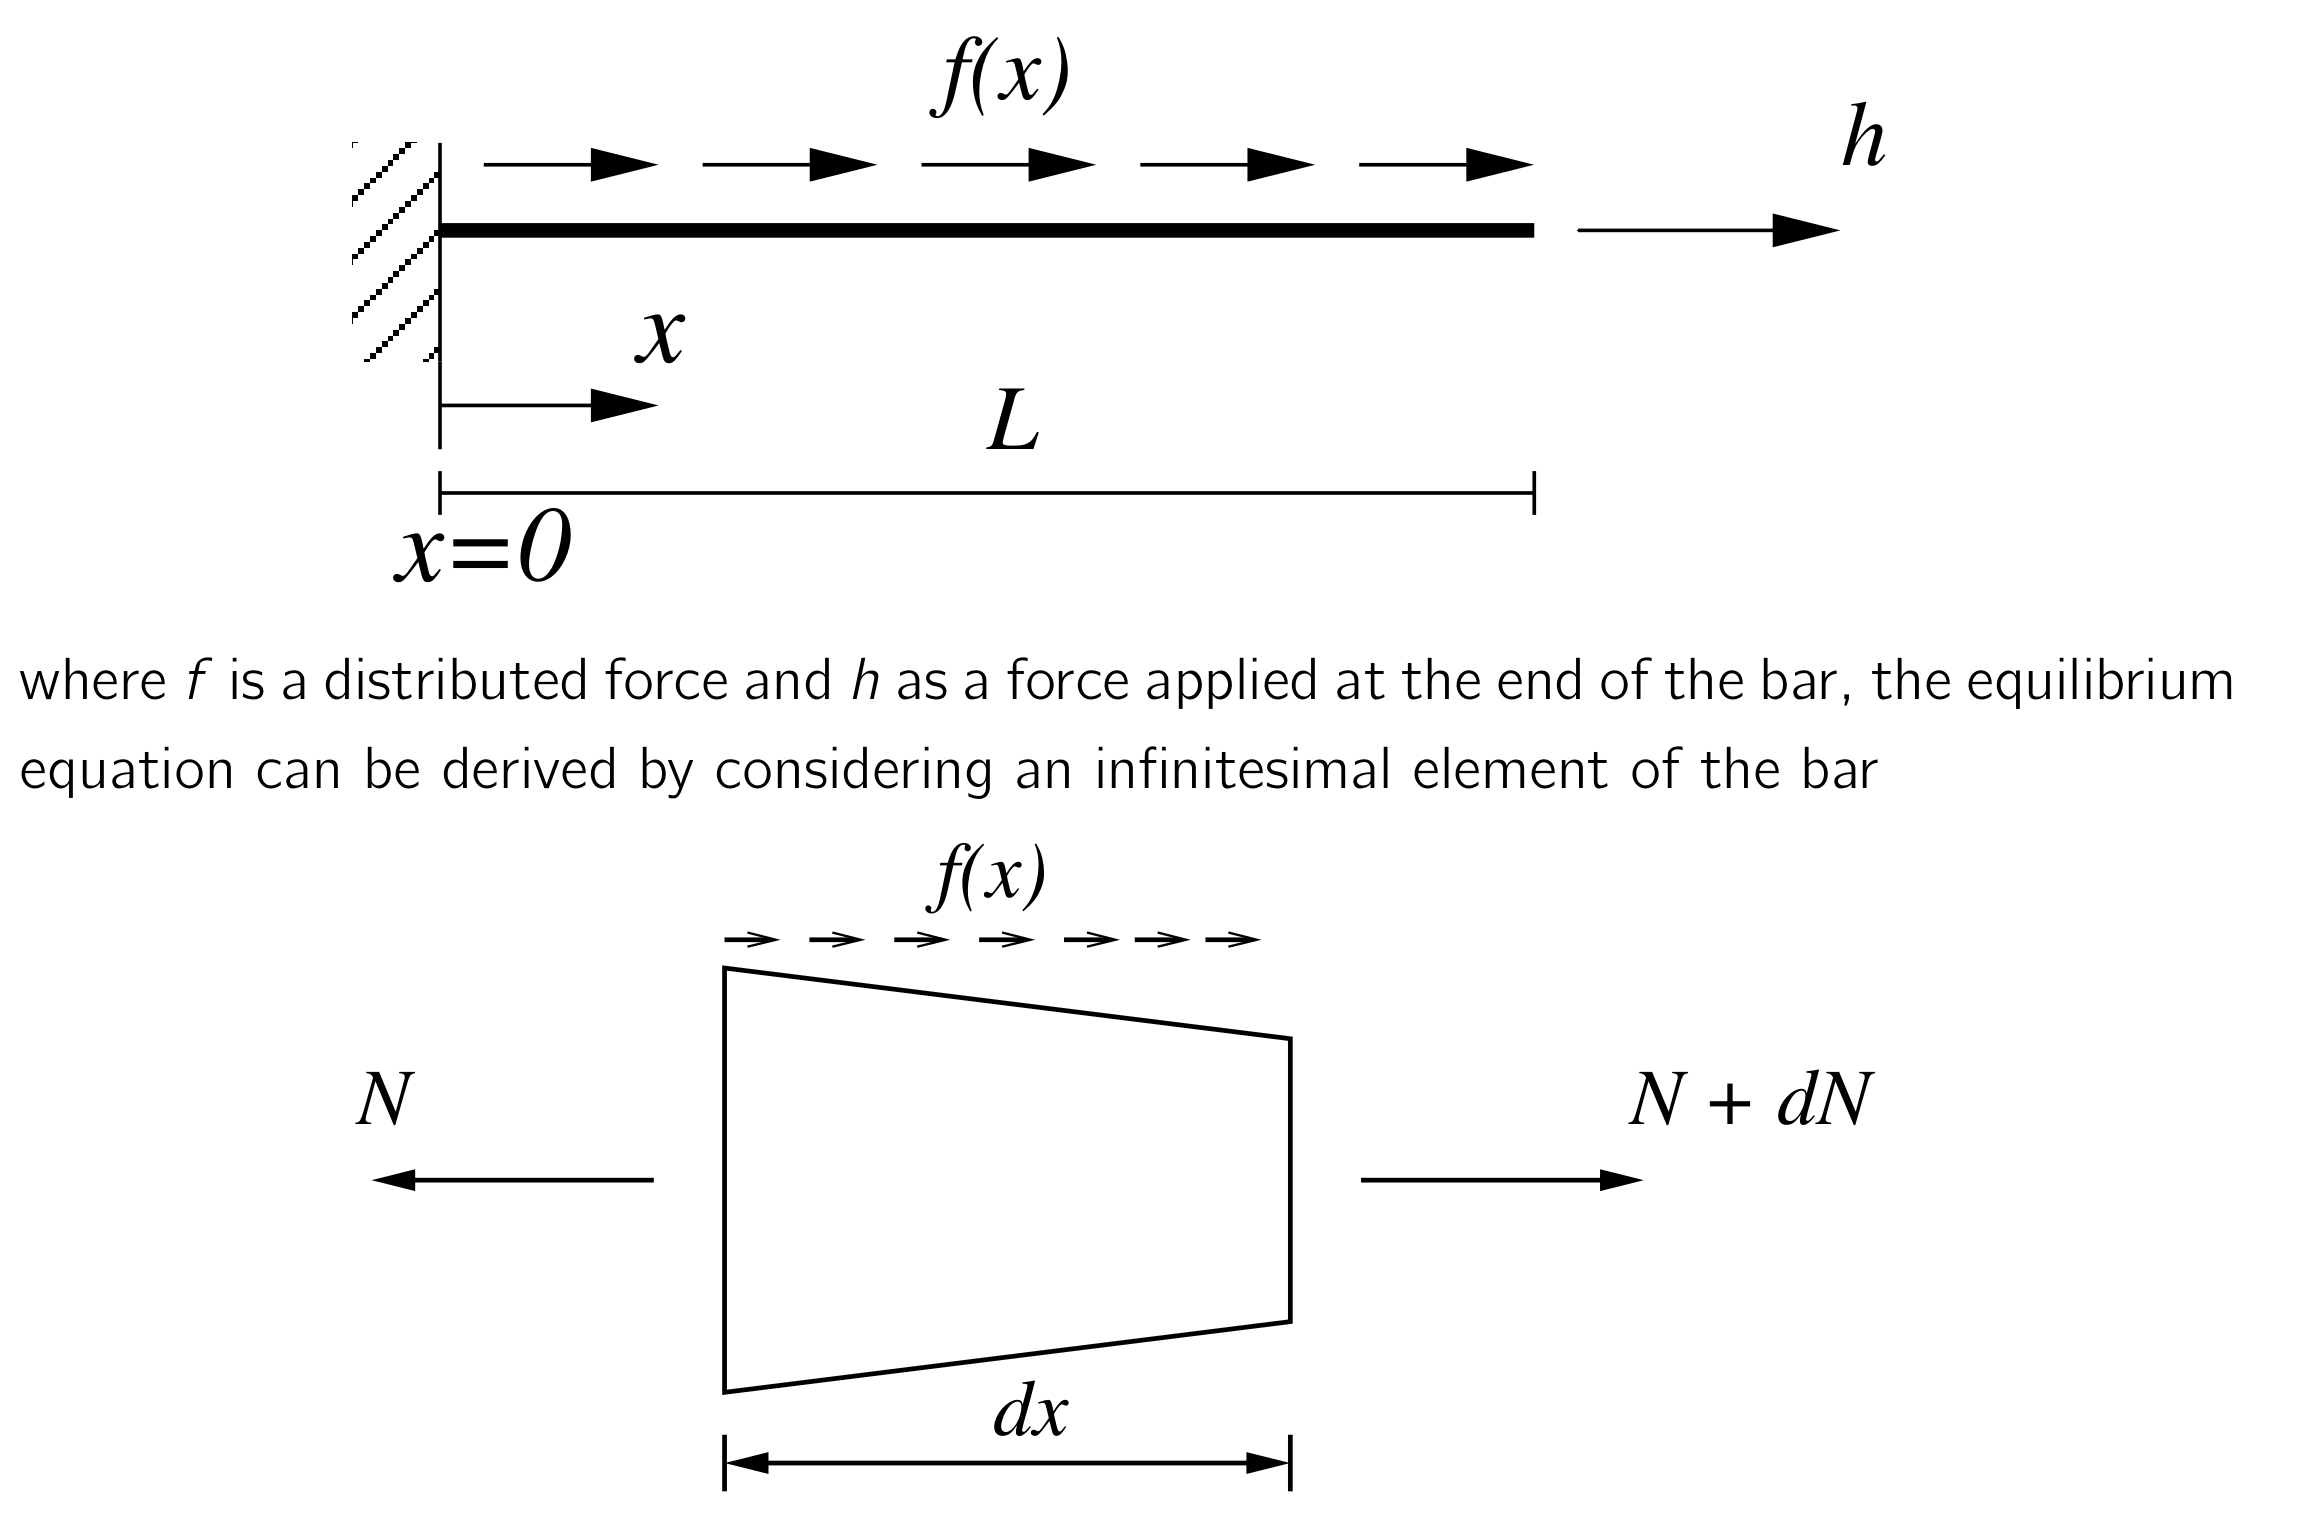
\includegraphics[width=\textwidth]{figs/strong-form-1d-bar.png}
	\caption*{where $f$ is a distributed force and $h$ as a force applied at the end of the bar}
\end{figure}
The equilibrium equation can be derived by considering an infinitesimal bar: 
\mode<beamer>{
	\begin{equation*}
		- \frac{dN}{dx} = f
	\end{equation*}
}
\mode<handout>{
	\vspace{2cm}
}
where $N$ is the normal force in the bar and $f$ is the distributed force along the bar.
\end{frame}

%------------------------------------------------
\begin{frame}
\frametitle{Boundary value problem of a 1-D bar}
For linear elasticity
\mode<beamer>{
	\begin{equation*}
		N = A \sigma = E A \frac{du}{dx} = EA\varepsilon
	\end{equation*}
}
\mode<handout>{
	\vspace{1.5cm}
}
where $A(x)$ is the area of the bar, $E(x)$ is Young’s modulus $u$ is the displacement and $\varepsilon =
du/dx$ is the strain.
\mode<beamer>{
	\begin{equation*}
	- \frac{d}{dx}\left(EA \frac{du}{dx}\right) = f
	\end{equation*}
}
\mode<handout>{
	\vspace{1.5cm}
}
which is a second-order differential equation. BCs:
\mode<beamer>{
	\begin{enumerate}
	\item $u = 0$ at $x = 0$ (displacement or `Dirichlet' boundary condition),
	\item $EA\varepsilon = h$ at $x = L$ (force or `Neumann' boundary condition).
	\end{enumerate}
We now have a well-defined boundary value problem that can be solved.
}
\mode<handout>{
	\vspace{1cm}
}


\end{frame}
\note{To formulate a boundary value problem, we need to assume a constitutive model which
	defines the relationship between stress and deformation, and we need to supply boundary
	conditions.}

% Strong vs Weak form
\note{Strong form is the conventional PDE. Weak form is an alternate representation of 
	the differential equation. The strong form imposes continuity and differentiability 
	requirements on the potential solutions to the equation. The weak form relaxes these 
	requirements on solutions to a certain extent. This means that a larger set of 
	functions are solutions of the weak form. By construction all solutions of the strong 
	form satisfy the weak form but not vice-versa. \\

	Weak formulations are often referred to as `variational formulations', but they they 
	can still be formulated for problems that cannot be phrased as a minimisation problem. 
	The weak form of an equation does not generally make an equation easier to solve 
	analytically (it may make it harder), but is usually a more suitable form for 
	mathematical analysis (allowing us to say things about the properties of the equation 
	without knowing the solution) and for numerical solution methods.}

\end{document} 
